\documentclass[]{article}
\usepackage{lmodern}
\usepackage{amssymb,amsmath}
\usepackage{ifxetex,ifluatex}
\usepackage{fixltx2e} % provides \textsubscript
\ifnum 0\ifxetex 1\fi\ifluatex 1\fi=0 % if pdftex
  \usepackage[T1]{fontenc}
  \usepackage[utf8]{inputenc}
\else % if luatex or xelatex
  \ifxetex
    \usepackage{mathspec}
  \else
    \usepackage{fontspec}
  \fi
  \defaultfontfeatures{Ligatures=TeX,Scale=MatchLowercase}
\fi
% use upquote if available, for straight quotes in verbatim environments
\IfFileExists{upquote.sty}{\usepackage{upquote}}{}
% use microtype if available
\IfFileExists{microtype.sty}{%
\usepackage{microtype}
\UseMicrotypeSet[protrusion]{basicmath} % disable protrusion for tt fonts
}{}
\usepackage[margin=1in]{geometry}
\usepackage{hyperref}
\hypersetup{unicode=true,
            pdftitle={Atlas-PS 8},
            pdfauthor={David Atlas},
            pdfborder={0 0 0},
            breaklinks=true}
\urlstyle{same}  % don't use monospace font for urls
\usepackage{color}
\usepackage{fancyvrb}
\newcommand{\VerbBar}{|}
\newcommand{\VERB}{\Verb[commandchars=\\\{\}]}
\DefineVerbatimEnvironment{Highlighting}{Verbatim}{commandchars=\\\{\}}
% Add ',fontsize=\small' for more characters per line
\usepackage{framed}
\definecolor{shadecolor}{RGB}{248,248,248}
\newenvironment{Shaded}{\begin{snugshade}}{\end{snugshade}}
\newcommand{\KeywordTok}[1]{\textcolor[rgb]{0.13,0.29,0.53}{\textbf{{#1}}}}
\newcommand{\DataTypeTok}[1]{\textcolor[rgb]{0.13,0.29,0.53}{{#1}}}
\newcommand{\DecValTok}[1]{\textcolor[rgb]{0.00,0.00,0.81}{{#1}}}
\newcommand{\BaseNTok}[1]{\textcolor[rgb]{0.00,0.00,0.81}{{#1}}}
\newcommand{\FloatTok}[1]{\textcolor[rgb]{0.00,0.00,0.81}{{#1}}}
\newcommand{\ConstantTok}[1]{\textcolor[rgb]{0.00,0.00,0.00}{{#1}}}
\newcommand{\CharTok}[1]{\textcolor[rgb]{0.31,0.60,0.02}{{#1}}}
\newcommand{\SpecialCharTok}[1]{\textcolor[rgb]{0.00,0.00,0.00}{{#1}}}
\newcommand{\StringTok}[1]{\textcolor[rgb]{0.31,0.60,0.02}{{#1}}}
\newcommand{\VerbatimStringTok}[1]{\textcolor[rgb]{0.31,0.60,0.02}{{#1}}}
\newcommand{\SpecialStringTok}[1]{\textcolor[rgb]{0.31,0.60,0.02}{{#1}}}
\newcommand{\ImportTok}[1]{{#1}}
\newcommand{\CommentTok}[1]{\textcolor[rgb]{0.56,0.35,0.01}{\textit{{#1}}}}
\newcommand{\DocumentationTok}[1]{\textcolor[rgb]{0.56,0.35,0.01}{\textbf{\textit{{#1}}}}}
\newcommand{\AnnotationTok}[1]{\textcolor[rgb]{0.56,0.35,0.01}{\textbf{\textit{{#1}}}}}
\newcommand{\CommentVarTok}[1]{\textcolor[rgb]{0.56,0.35,0.01}{\textbf{\textit{{#1}}}}}
\newcommand{\OtherTok}[1]{\textcolor[rgb]{0.56,0.35,0.01}{{#1}}}
\newcommand{\FunctionTok}[1]{\textcolor[rgb]{0.00,0.00,0.00}{{#1}}}
\newcommand{\VariableTok}[1]{\textcolor[rgb]{0.00,0.00,0.00}{{#1}}}
\newcommand{\ControlFlowTok}[1]{\textcolor[rgb]{0.13,0.29,0.53}{\textbf{{#1}}}}
\newcommand{\OperatorTok}[1]{\textcolor[rgb]{0.81,0.36,0.00}{\textbf{{#1}}}}
\newcommand{\BuiltInTok}[1]{{#1}}
\newcommand{\ExtensionTok}[1]{{#1}}
\newcommand{\PreprocessorTok}[1]{\textcolor[rgb]{0.56,0.35,0.01}{\textit{{#1}}}}
\newcommand{\AttributeTok}[1]{\textcolor[rgb]{0.77,0.63,0.00}{{#1}}}
\newcommand{\RegionMarkerTok}[1]{{#1}}
\newcommand{\InformationTok}[1]{\textcolor[rgb]{0.56,0.35,0.01}{\textbf{\textit{{#1}}}}}
\newcommand{\WarningTok}[1]{\textcolor[rgb]{0.56,0.35,0.01}{\textbf{\textit{{#1}}}}}
\newcommand{\AlertTok}[1]{\textcolor[rgb]{0.94,0.16,0.16}{{#1}}}
\newcommand{\ErrorTok}[1]{\textcolor[rgb]{0.64,0.00,0.00}{\textbf{{#1}}}}
\newcommand{\NormalTok}[1]{{#1}}
\usepackage{graphicx,grffile}
\makeatletter
\def\maxwidth{\ifdim\Gin@nat@width>\linewidth\linewidth\else\Gin@nat@width\fi}
\def\maxheight{\ifdim\Gin@nat@height>\textheight\textheight\else\Gin@nat@height\fi}
\makeatother
% Scale images if necessary, so that they will not overflow the page
% margins by default, and it is still possible to overwrite the defaults
% using explicit options in \includegraphics[width, height, ...]{}
\setkeys{Gin}{width=\maxwidth,height=\maxheight,keepaspectratio}
\IfFileExists{parskip.sty}{%
\usepackage{parskip}
}{% else
\setlength{\parindent}{0pt}
\setlength{\parskip}{6pt plus 2pt minus 1pt}
}
\setlength{\emergencystretch}{3em}  % prevent overfull lines
\providecommand{\tightlist}{%
  \setlength{\itemsep}{0pt}\setlength{\parskip}{0pt}}
\setcounter{secnumdepth}{0}
% Redefines (sub)paragraphs to behave more like sections
\ifx\paragraph\undefined\else
\let\oldparagraph\paragraph
\renewcommand{\paragraph}[1]{\oldparagraph{#1}\mbox{}}
\fi
\ifx\subparagraph\undefined\else
\let\oldsubparagraph\subparagraph
\renewcommand{\subparagraph}[1]{\oldsubparagraph{#1}\mbox{}}
\fi

%%% Use protect on footnotes to avoid problems with footnotes in titles
\let\rmarkdownfootnote\footnote%
\def\footnote{\protect\rmarkdownfootnote}

%%% Change title format to be more compact
\usepackage{titling}

% Create subtitle command for use in maketitle
\newcommand{\subtitle}[1]{
  \posttitle{
    \begin{center}\large#1\end{center}
    }
}

\setlength{\droptitle}{-2em}
  \title{Atlas-PS 8}
  \pretitle{\vspace{\droptitle}\centering\huge}
  \posttitle{\par}
  \author{David Atlas}
  \preauthor{\centering\large\emph}
  \postauthor{\par}
  \predate{\centering\large\emph}
  \postdate{\par}
  \date{10/21/2018}


\begin{document}
\maketitle

\newcommand{\summ}{\sum_{i=1}^n}



\section{Problem 1}\label{problem-1}

First, we read in the dataset for the problem.

\begin{Shaded}
\begin{Highlighting}[]
\NormalTok{x <-}\StringTok{ }\KeywordTok{scan}\NormalTok{(}\StringTok{"xvalues.txt"}\NormalTok{)}
\NormalTok{y <-}\StringTok{ }\KeywordTok{scan}\NormalTok{(}\StringTok{"yvalues.txt"}\NormalTok{)}
\end{Highlighting}
\end{Shaded}

\subsection{a)}\label{a}

First, we plot the data.

\begin{Shaded}
\begin{Highlighting}[]
\KeywordTok{plot}\NormalTok{(x, y, }\DataTypeTok{main=}\StringTok{"X vs. Y"}\NormalTok{)}
\end{Highlighting}
\end{Shaded}

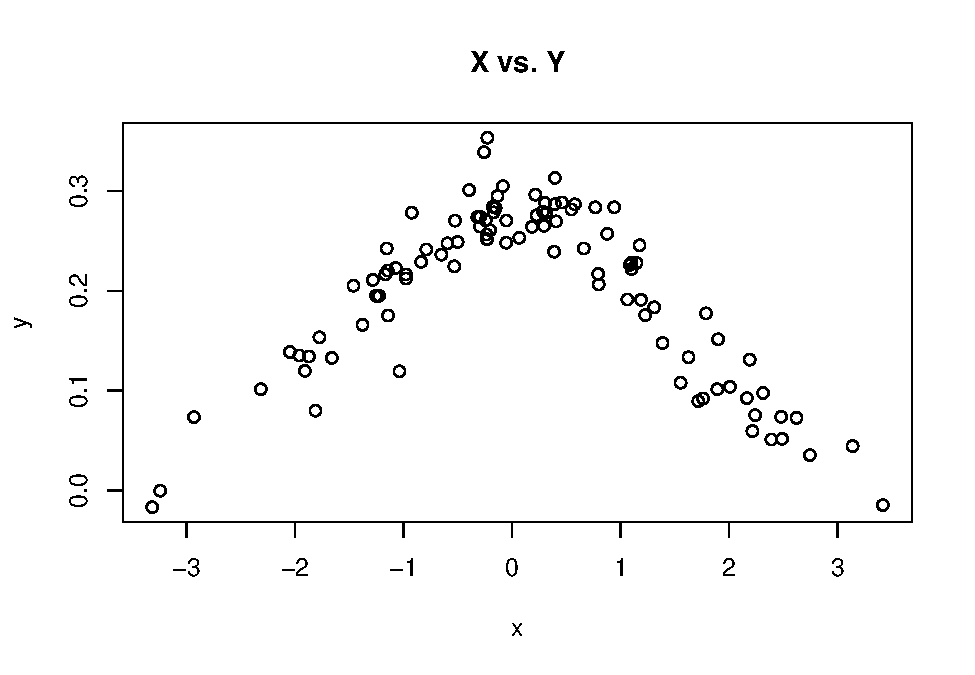
\includegraphics{Atlas-PS_8_files/figure-latex/unnamed-chunk-2-1.pdf}

The MLE of the mean of the distribution is simply the observed mean of
X, so we can easily find it.

\begin{Shaded}
\begin{Highlighting}[]
\NormalTok{mu <-}\StringTok{ }\KeywordTok{mean}\NormalTok{(x)}
\KeywordTok{print}\NormalTok{(}\KeywordTok{round}\NormalTok{(mu, }\DecValTok{3}\NormalTok{))}
\end{Highlighting}
\end{Shaded}

\begin{verbatim}
## [1] 0.173
\end{verbatim}

We use the to parameterize \(g\). We can say \[
g(x) = \frac{1}{\sqrt{4 \pi}}\rm{e}^{-\frac{(x - .173)^2}{4}},
\] which is the normal density with \(\mu = .173\) and \(\sigma^2 = 2\).

We can find the apparent error below:

\begin{Shaded}
\begin{Highlighting}[]
\KeywordTok{mean}\NormalTok{(}\KeywordTok{abs}\NormalTok{(y -}\StringTok{ }\KeywordTok{dnorm}\NormalTok{(x, }\KeywordTok{mean}\NormalTok{(x), }\KeywordTok{sqrt}\NormalTok{(}\DecValTok{2}\NormalTok{))))}
\end{Highlighting}
\end{Shaded}

\begin{verbatim}
## [1] 0.02518254
\end{verbatim}

The mean absolute error is .025.

\subsection{b)}\label{b}

Next, we partition our dataset into 2 halves, and repeat the process.

\begin{Shaded}
\begin{Highlighting}[]
\NormalTok{x_1 <-}\StringTok{ }\NormalTok{x[}\DecValTok{1}\NormalTok{:}\DecValTok{50}\NormalTok{]}
\NormalTok{x_2 <-}\StringTok{ }\NormalTok{x[}\DecValTok{50}\NormalTok{:}\DecValTok{100}\NormalTok{]}

\NormalTok{y_1 <-}\StringTok{ }\NormalTok{y[}\DecValTok{1}\NormalTok{:}\DecValTok{50}\NormalTok{]}
\NormalTok{y_2 <-}\StringTok{ }\NormalTok{y[}\DecValTok{50}\NormalTok{:}\DecValTok{100}\NormalTok{]}

\CommentTok{# Find the predicted values of y }
\NormalTok{e_1 <-}\StringTok{ }\KeywordTok{abs}\NormalTok{(y_1 -}\StringTok{ }\KeywordTok{dnorm}\NormalTok{(x_1, }\KeywordTok{mean}\NormalTok{(x_2), }\KeywordTok{sqrt}\NormalTok{(}\DecValTok{2}\NormalTok{)))}
\NormalTok{e_2 <-}\StringTok{ }\KeywordTok{abs}\NormalTok{(y_2 -}\StringTok{ }\KeywordTok{dnorm}\NormalTok{(x_2, }\KeywordTok{mean}\NormalTok{(x_1), }\KeywordTok{sqrt}\NormalTok{(}\DecValTok{2}\NormalTok{)))}

\KeywordTok{print}\NormalTok{(}\KeywordTok{round}\NormalTok{(}\KeywordTok{mean}\NormalTok{(e_1) +}\StringTok{ }\KeywordTok{mean}\NormalTok{(e_2), }\DecValTok{3}\NormalTok{))}
\end{Highlighting}
\end{Shaded}

\begin{verbatim}
## [1] 0.061
\end{verbatim}

The out of sample error is .061

\subsection{c)}\label{c}

This is what one might expect. The error is lower when calculated on
data points that were included in the fit of the function. When we fit
on one partition and calculate the error on the other partition, we find
that there is a much higher error.

\section{Problem 2}\label{problem-2}

\subsection{a)}\label{a-1}

To show the equality in the problem, we establish a few equalities from
the text (Gentle).

\begin{align}
T^*_j &= nT - (n-1)T_{-j} \\
J(T) &= nT - (n-1) \overline{T}_{(\cdot)}.
\end{align}

Therefore, we can say that

\begin{align*}
\summ(T^*_j - J(T))^2 &= \summ(nT - (n-1)T_{-j} - nT + (n-1)\overline{T}_{(\cdot)} )^2 \\
&= \summ(- (n-1)T_{-j} + (n-1) \overline{T}_{(\cdot)})^2 \\
&= \summ(n-1)^2 (-T_{-j} + \overline{T}_{(\cdot)})^2.
\end{align*}

Note that \((a - b)^2 = (b -a)^2\), so we can say that \[
\summ(n-1)^2 (-T_{-j} + \overline{T}_{(\cdot)})^2 = (n-1)^2 \summ (T_{-j} - \overline{T}_{(\cdot)})^2.
\]

At this point, we can say that \[
\frac{\summ(T^*_j - J(T))^2 }{n (n-1)} = \frac{n-1}{n}\summ(T_{-j} - \overline{T}_{(\cdot)})^2.
\]

\subsection{b)}\label{b-1}

To show that
\(\widehat{V(T)}_J \leq \frac{\summ (T^*_j - T)^2}{n(n-1)}\), where
\(\widehat{V(T)}_J = \frac{\summ (T^*_j - J(T))^2}{n(n-1)}\), we note
that the minimization of the function \(f(z) = \summ(x_i - z)^2\), for
any set of observations \((x_1, \ldots, x_n)\), is equal to
\(\bar{x} = \frac{1}{n}\summ{x_i}\).

This can be shown by taking the first derivative of \(f(z)\), \[
f^\prime(z) = -2 \summ(T^*_j - z).
\]

Setting it equal to zero and solving,

\begin{align*}
&-2 \summ(T^*_j - z) = 0 \\
&\implies \summ T^*_j = nz  \\
&\implies z = \frac{\summ T^*_j}{n}.
\end{align*}

Therefore, \(\summ (T^*_j - J(T))^2 \leq \summ (T^*_j - z)^2\),
\(\forall z \in \mathbb{R}\). By extension,
\(\frac{\summ (T^*_j - J(T))^2 \leq}{n(n-1)} \leq \frac{\summ (T^*_j - T)^2 }{n(n-1)}\).

\section{Problem 3}\label{problem-3}

\subsection{a)}\label{a-2}

Let \(b_{2, -j}\) be the calculation of \(b_2\) having removed the
\(j^{\rm{th}}\) jackknife of the dataset.

The jackknife estimate of the variance (from Gentle) is \[
\widehat{V(b_2)_J} = \frac{\sum_{j=1}^r (r b_2 - (r - 1) b_{2, j} -    \sum_{j=1}^r (r b_2 - (r - 1) b_{2, j}    ))^2  }{r (r -1)}.
\]

The standard deviation is simply the square root of
\(\widehat{V(b_2)_J}\).

\subsection{b)}\label{b-2}

Next, we use the datapoints on Blackboard to find \(b_2\) and the
jackknife estimate of the standard deviation for the cases \(k=1\) and
\(k=5\).

We read in the data, and define the calculation of \(b_2\).

\begin{Shaded}
\begin{Highlighting}[]
\NormalTok{jackknife <-}\StringTok{ }\KeywordTok{scan}\NormalTok{(}\StringTok{"./Module 8 Data Sets/Jackknife.txt"}\NormalTok{)}
\NormalTok{b2 <-}\StringTok{ }\NormalTok{function(y)\{}
  \NormalTok{ybar <-}\StringTok{ }\KeywordTok{mean}\NormalTok{(y)}
  \KeywordTok{return}\NormalTok{(}\KeywordTok{sum}\NormalTok{((y -}\StringTok{ }\NormalTok{ybar)^}\DecValTok{4}\NormalTok{) /}\StringTok{ }\NormalTok{(}\KeywordTok{sum}\NormalTok{((y -}\StringTok{ }\NormalTok{ybar)^}\DecValTok{2}\NormalTok{))^}\DecValTok{2}\NormalTok{)}
\NormalTok{\}}
\end{Highlighting}
\end{Shaded}

Next, we find the statistic over the whole dataset.

\begin{Shaded}
\begin{Highlighting}[]
\KeywordTok{round}\NormalTok{(}\KeywordTok{b2}\NormalTok{(jackknife), }\DecValTok{4}\NormalTok{)}
\end{Highlighting}
\end{Shaded}

\begin{verbatim}
## [1] 0.0267
\end{verbatim}

The value of \(b_2\) is .0267 over the entire sample.

Next, we find the jackknife estimate for the standard deviation of
\(b_{2}\) for \(k=1\).

\begin{Shaded}
\begin{Highlighting}[]
\NormalTok{t_star <-}\StringTok{ }\NormalTok{function(data, T, k)\{}
  \NormalTok{idx <-}\StringTok{ }\KeywordTok{split}\NormalTok{(}\KeywordTok{seq_along}\NormalTok{(data), }\KeywordTok{ceiling}\NormalTok{(}\KeywordTok{seq_along}\NormalTok{(data) /}\StringTok{  }\NormalTok{k))}
  \NormalTok{r <-}\StringTok{ }\KeywordTok{length}\NormalTok{(data) /}\StringTok{ }\NormalTok{k}
  \KeywordTok{return}\NormalTok{(}\KeywordTok{sapply}\NormalTok{(idx, function(id)\{}
    \KeywordTok{return}\NormalTok{(r *}\StringTok{ }\KeywordTok{T}\NormalTok{(data) -}\StringTok{ }\NormalTok{(r -}\DecValTok{1}\NormalTok{) *}\StringTok{ }\KeywordTok{T}\NormalTok{(data[-id]))}
  \NormalTok{\}))}
\NormalTok{\}}

\NormalTok{J <-}\StringTok{ }\NormalTok{function(data, T, k)\{}
  \KeywordTok{mean}\NormalTok{(}\KeywordTok{t_star}\NormalTok{(data, T, k))}
\NormalTok{\}}

\NormalTok{var_t <-}\StringTok{ }\NormalTok{function(data, T, k)\{}
  \NormalTok{tstar <-}\StringTok{ }\KeywordTok{t_star}\NormalTok{(data, T, k)}
  \NormalTok{j <-}\StringTok{ }\KeywordTok{J}\NormalTok{(data, T, k)}
  \NormalTok{r <-}\StringTok{ }\KeywordTok{length}\NormalTok{(data) /}\StringTok{ }\NormalTok{k}
  \KeywordTok{return}\NormalTok{(}\KeywordTok{sum}\NormalTok{((tstar -}\StringTok{ }\NormalTok{j)^}\DecValTok{2}\NormalTok{) /}\StringTok{ }\NormalTok{(r *}\StringTok{ }\NormalTok{(r}\DecValTok{-1}\NormalTok{)))}
\NormalTok{\}}


\KeywordTok{sqrt}\NormalTok{(}\KeywordTok{var_t}\NormalTok{(jackknife, b2, }\DecValTok{1}\NormalTok{))}
\end{Highlighting}
\end{Shaded}

\begin{verbatim}
## [1] 0.003714044
\end{verbatim}

The jackknife estimate of the standard deviation of \(b_2\) when \(k=1\)
is .00371.

Next, we try again with \(k=5\).

\begin{Shaded}
\begin{Highlighting}[]
\KeywordTok{sqrt}\NormalTok{(}\KeywordTok{var_t}\NormalTok{(jackknife, b2, }\DecValTok{5}\NormalTok{))}
\end{Highlighting}
\end{Shaded}

\begin{verbatim}
## [1] 0.003692711
\end{verbatim}

The jackknife estimate of the standard deviation of \(b_2\) when \(k=5\)
is .00369.

\subsection{c)}\label{c-1}

To get a sense for the actual standard deviation of \(b_2\), we generate
several samples from a \(N(0, 1)\) distribution.

\begin{Shaded}
\begin{Highlighting}[]
\KeywordTok{set.seed}\NormalTok{(}\DecValTok{73}\NormalTok{)}
\KeywordTok{sd}\NormalTok{(}\KeywordTok{sapply}\NormalTok{(}\KeywordTok{seq}\NormalTok{(}\DecValTok{1}\NormalTok{, }\DecValTok{10000}\NormalTok{), function(i)\{}
  \NormalTok{b2_hat <-}\StringTok{ }\KeywordTok{b2}\NormalTok{(}\KeywordTok{rnorm}\NormalTok{(}\KeywordTok{length}\NormalTok{(jackknife), }\DecValTok{0}\NormalTok{, }\DecValTok{1}\NormalTok{))}
\NormalTok{\}))}
\end{Highlighting}
\end{Shaded}

\begin{verbatim}
## [1] 0.004568534
\end{verbatim}

Using samples of the same size as the dataset that we read in, we see
that the standard deviation observed is actually greater than the
jackknifed estimate of the standard deviation. The percent error of the
estimator relative to that of the sampled data is about 23\%.

Therefore, the estimator does not perform well, as it underestimates the
variance seen, which can lead to incorrect inference on the data.


\end{document}
